\documentclass[a4paper,12pt]{article} % добавить leqno в [] для нумерации слева
\usepackage[a4paper,top=1.3cm,bottom=2cm,left=1.5cm,right=1.5cm,marginparwidth=0.75cm]{geometry}
%%% Работа с русским языком
\usepackage{cmap}					% поиск в PDF
\usepackage[warn]{mathtext} 		% русские буквы в фомулах
\usepackage[T2A]{fontenc}			% кодировка
\usepackage[utf8]{inputenc}			% кодировка исходного текста
\usepackage[english,russian]{babel}	% локализация и переносы
\usepackage{physics}
\usepackage{multirow}
\usepackage{bm}
\usepackage{longtable}
\usepackage{xcolor}
%%% Нормальное размещение таблиц (писать [H] в окружении таблицы)
\usepackage{float}
\restylefloat{table}


\usepackage[utf8]{inputenc}
\usepackage[russian]{babel}
\usepackage{amsmath}
\usepackage{amssymb}
\usepackage{graphicx}
\usepackage{geometry}
\usepackage{booktabs}
\usepackage{caption}
\usepackage{enumitem}
\usepackage{siunitx}

\geometry{left=2cm,right=1.5cm,top=2cm,bottom=2cm}
\setlist[enumerate]{label=\arabic*., leftmargin=*}


\usepackage{graphicx}

\usepackage{wrapfig}
\usepackage{tabularx}

\usepackage{hyperref}
\usepackage[rgb]{xcolor}
\hypersetup{
	colorlinks=true,urlcolor=blue
}
\usepackage{pgfplots}
\pgfplotsset{compat=1.9}
%%% Дополнительная работа с математикой
\usepackage{amsmath,amsfonts,amssymb,amsthm,mathtools} % AMS
\usepackage{icomma} % "Умная" запятая: $0,2$ --- число, $0, 2$ --- перечисление

%% Номера формул
%\mathtoolsset{showonlyrefs=true} % Показывать номера только у тех формул, на которые есть \eqref{} в тексте,

%% Шрифты
\usepackage{euscript}	 % Шрифт Евклид
\usepackage{mathrsfs} % Красивый матшрифт


\title{Архитектура вычислительных систем. Домашнее задание №2. Вариант №1.}
\author{Комиссаров Данил Андреевич}
\date{March 2025}

\begin{document}

\maketitle

\section{Полный отчет}
Первый вариант задания. Арифметико-логическое устройство (ALU).

В отличие от предыдущего задания, где достаточно было школьной логики и курса дискретного анализа, здесь требуется умение работы с Verilog, что среди студентов второго курса не является очень распространённым. Поэтому сначала будет уместно разобраться с языком описания аппаратуры с нуля.

К счастью, это удобно разбирать на примере АЛУ, который и сам состоит из простых элементов: сумматор, компаратор, многобитные логические элементы. Постепенно их создавая, придём к полному пониманию языка. 

\subsection{Разбор}
Что вообще представляет собой так называемый модуль \textbf{"alu\_register"}?
Вообще это некий блок, который под управлением устройства управления служит для выполнения арифметических и логических преобразований над данными, называемыми в этом случае операндами. Разрядность операндов обычно называют размером или длиной машинного слова. То есть из себя АЛУ представляет несколько блоков комбинационной логики, которые и являются преобразованиями над операндами, и блока коммутатора, который соединяет соответствующий блок с выходом в зависимости от сигнала инструкций. 
В ТЗ описаны следующие команды:
\begin{figure}[H]
    \centering
    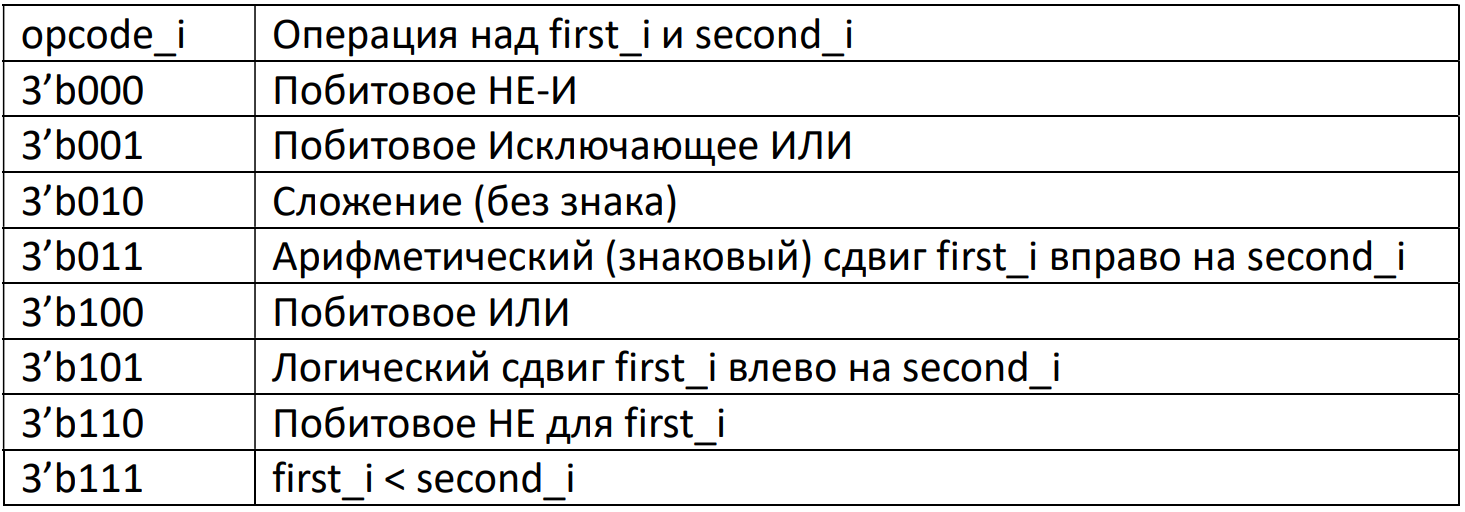
\includegraphics[width=1\linewidth]{Intro/Commands.png}
\end{figure}
Тогда схематично можно так представить себе АЛУ:
\begin{figure}[H]
    \centering
    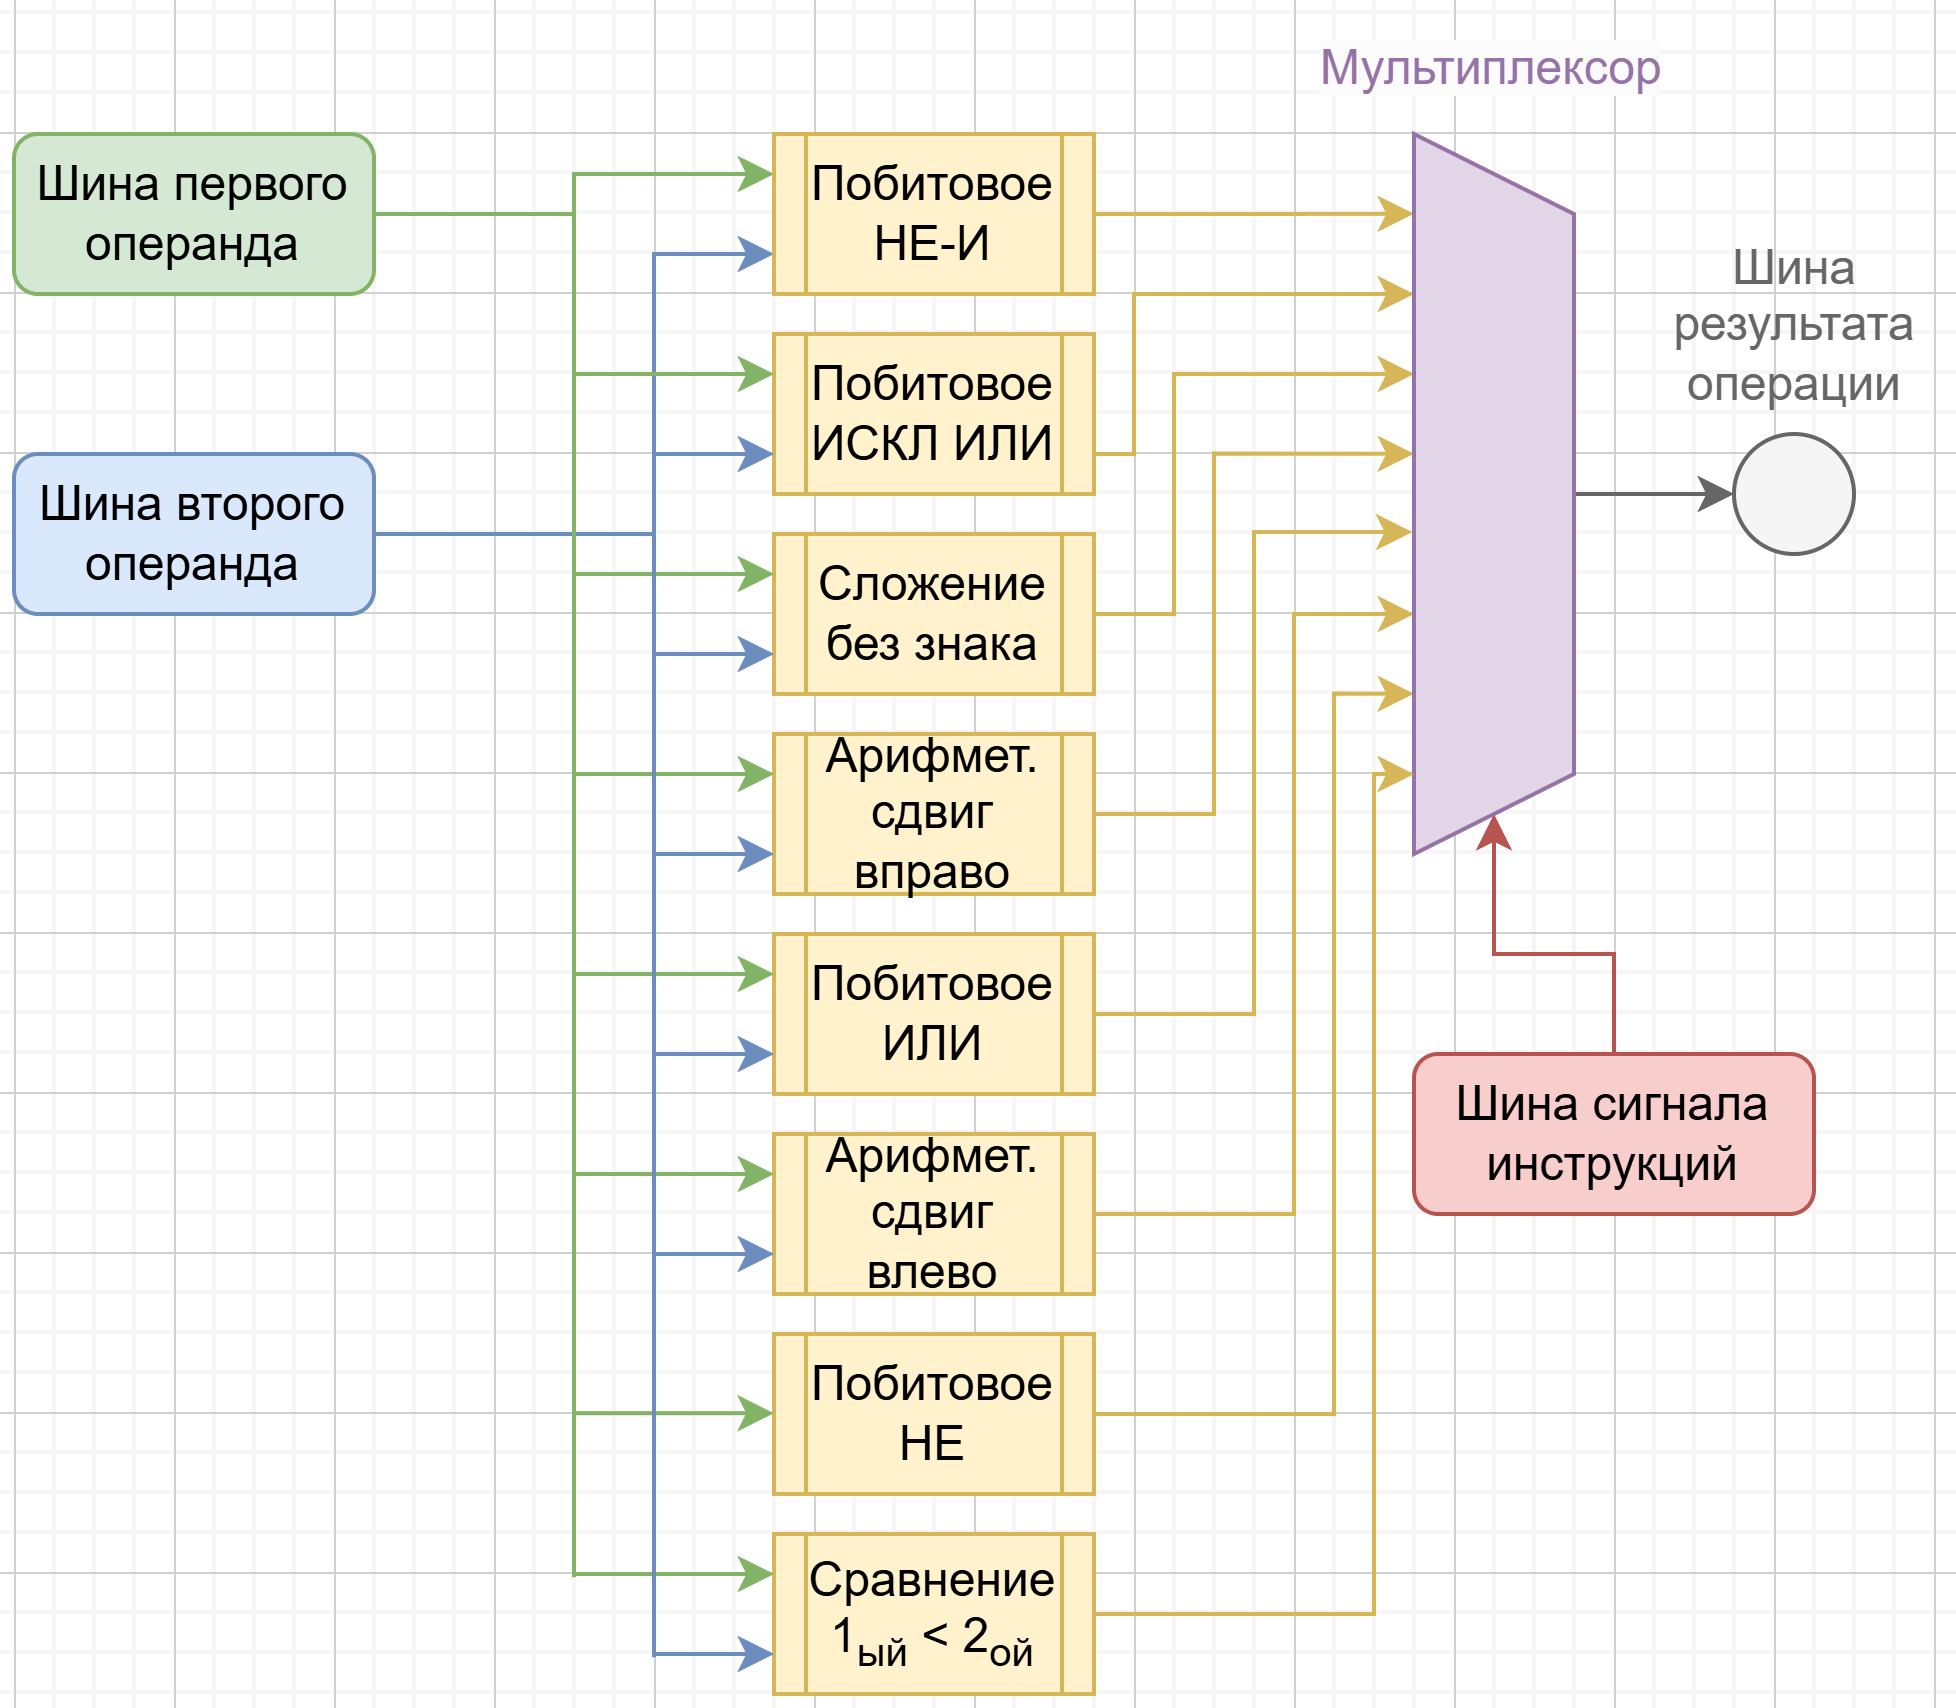
\includegraphics[width=1\linewidth]{Intro/АЛУ.png}
\end{figure}
Помимо прочего, вот следующие требования:
\begin{figure}[H]
    \centering
    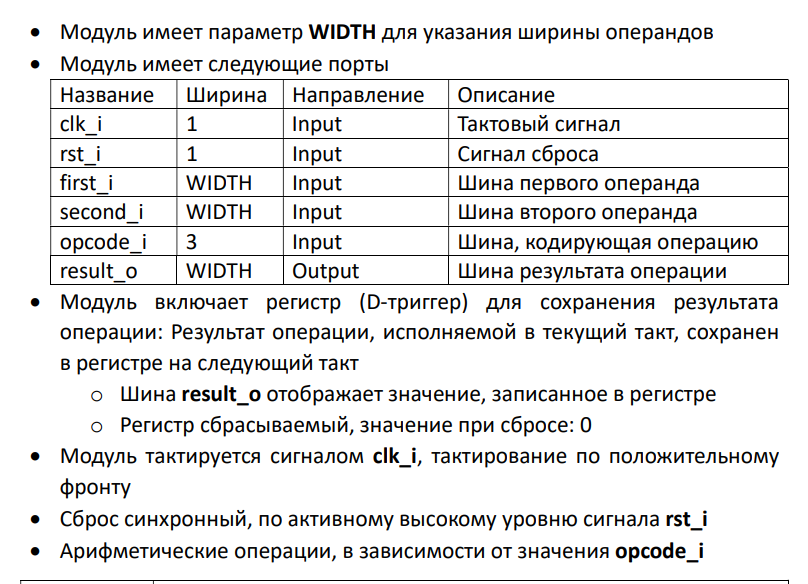
\includegraphics[width=1\linewidth]{Intro/ТЗ.png}
\end{figure}
То есть стоило бы переназвать элементы и добавить в принципиальную схему сигнал сброса и тактовый сигнал:
\begin{figure}[H]
    \centering
    \includegraphics[width=1\linewidth]{Intro/АЛУ1.png}
\end{figure}
Такова принципиальная схема, она понятна и проста, теперь можно переходить к следующему этапу.
\subsection{Verilog}
\subsubsection{Модули}

Программа на Verilog, она же описание схемы, состоит из модулей (module), точнее из экземпляров модулей (module instances). Модуль можно представить как “черный ящик” с торчащими из него проводами — портами (ports). Порты бывают трех типов: входные (input), выходные (output) и двунаправленные (inout). В большинстве случаев используются первые два типа портов. Двунаправленные порты нужны для моделирования двунаправленных шин, на базе выходов с тремя состояниями и открытым стоком. Их мы рассматривать не будем.

Список портов описывается в заголовке модуля. К примеру, рассмотрим этот пустой модуль:
\begin{figure}[H]
    \centering
    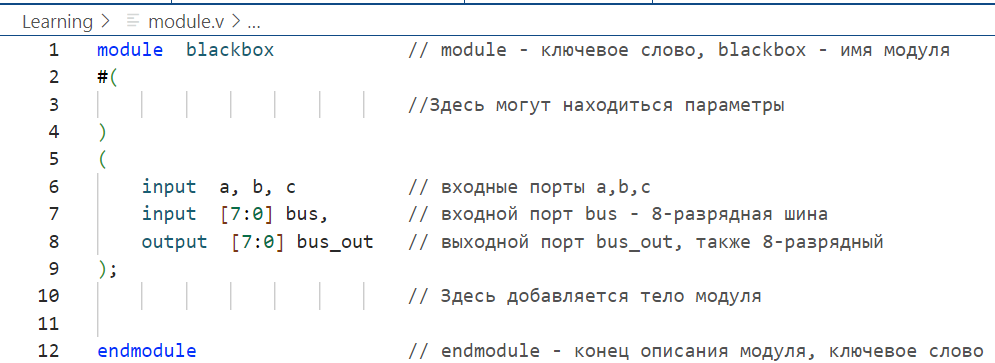
\includegraphics[width=1\linewidth]{Learning/module.png}
    \caption{\textbackslash Learning\textbackslash module.v}
\end{figure}

В теле модуля описывается его функциональность. Этот модуль пустой, его порты никуда не подключены.
\subsubsection{Типы данных}

В Verilog существуют два класса типов: типы для моделирования аппаратуры и стандартные арифметические типы данных, скопированные из языка Си. Рассмотрим первый класс, т.к. именно он используется для моделирования сигналов в схеме.

Сигнал может принимать 4 значения:
\begin{itemize}
    \item 0 – логический ноль, или ложь
    \item 1 – логическая единица, или истина
    \item x – неопределенное значение. К примеру, значение регистра в начальный момент симуляции (до сброса или первой записи в регистр)
    \item z – состояние с высоким импедансом. Чаще всего сигнал принимает это значение, если он никуда не подключен – “обрыв провода”
\end{itemize}

В большинстве модулей на Verilog используются 2 основных типа данных – \textbf{wire} и \textbf{reg}. Из названия может показаться, что \textbf{wire} моделирует провод, а \textbf{reg} – регистр, но, как будет показано далее, это не совсем так. Хотя и в SystemVerilog есть универсальный тип logic, который может использоваться во всех случаях.

\subsubsection{Wire}

Тип wire служит для моделирования сигналов, которые не могут “хранить” состояние. К примеру, значение на выходе комбинационной схемы полностью определяется значениями на входах. Если значения на входе меняются, меняется и значение на выходе, т.е. состояние не хранится.

Тип \textbf{wire} используется вместе с операцией непрерывного присваивания — \textbf{assign}. При непрерывном присваивании всякий раз, когда меняется значение переменных в правой части присваивания, обновляется значение переменной в левой части. К примеру, простую комбинационную схему можно описать следующим образом:
\begin{figure}[H]
    \centering
    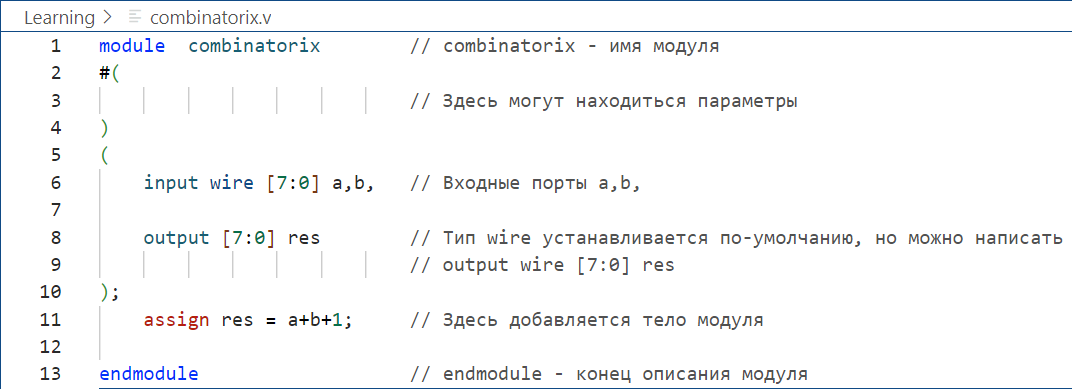
\includegraphics[width=1\linewidth]{Learning/combinatorix.png}
    \caption{\textbackslash Learning\textbackslash combinatorix.v}
\end{figure}
\begin{figure}[H]
    \centering
    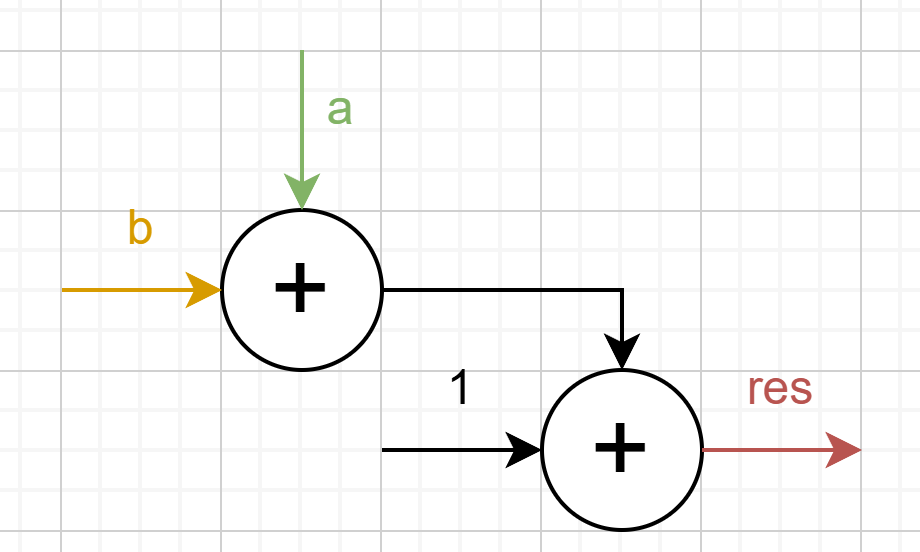
\includegraphics[width=0.75\linewidth]{Learning/combinatorix1.png}
\end{figure}
Если сигнал не объявлен явно (например, через reg или wire), он автоматически считается wire.
То есть действительно сущность \textbf{wire} можно принять за некоторый участок проводов. 

В коде было использовано так называемое \textit{непрерывное прививание} $"assign \dotsc = \dotsc "$. Это присваивание работает непрерывно, если проводить аналогию, то можно это представить как накоротко соединенный провод. Значение сигнала обновляется мгновенно при изменении любого из входных сигналов в правой части выражения. Целью присваивания всегда является сигнал типа \textbf{wire}. Нельзя использовать \textbf{assign} для переменных типа \textbf{reg}. 

\textbf{assign} используется для описания логических операций (AND, OR, сложение и т.д.), мультиплексоров, декодеров и других элементов без памяти.

\begin{figure}[H]
    \centering
    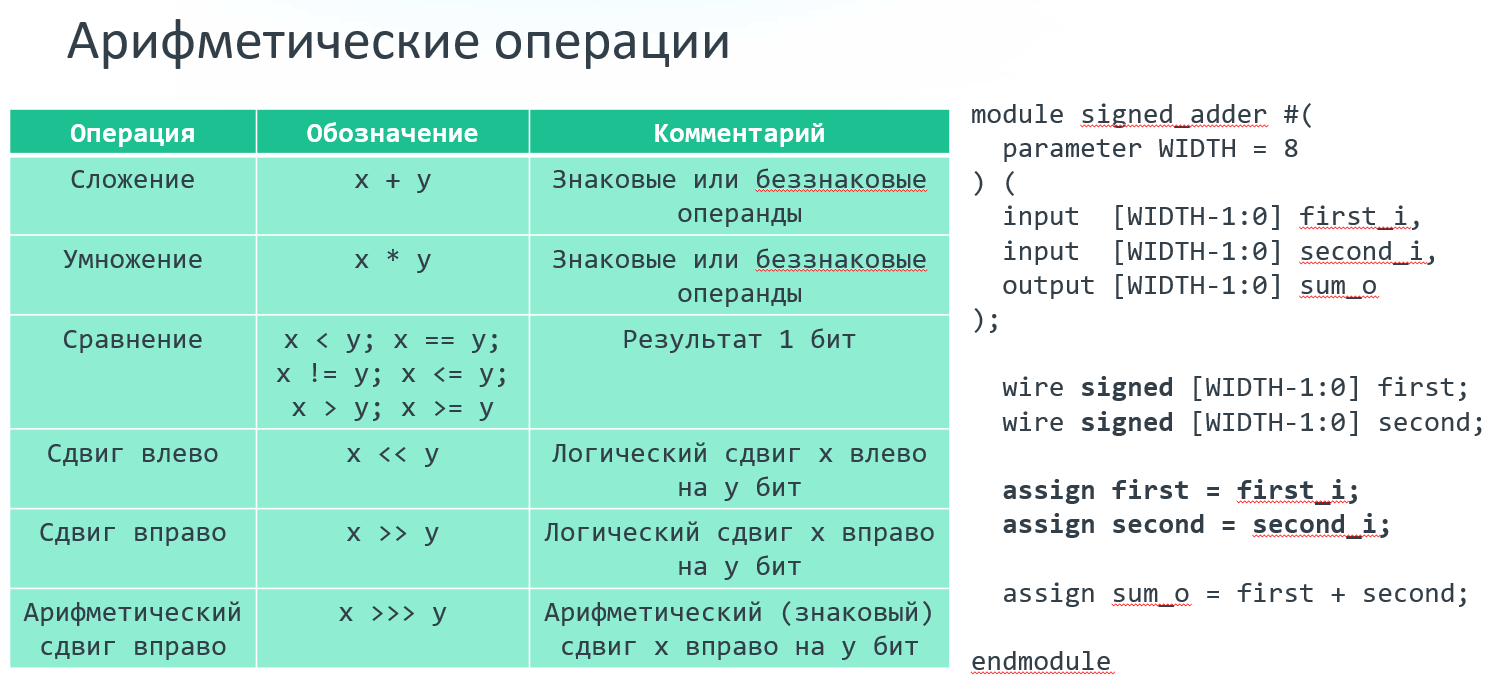
\includegraphics[width=1\linewidth]{Learning/table.png}
\end{figure}

Кстати о $"\text{[ ]}"$ перед именем переменной. Квадратные скобки используются для указания разрядности (битовой ширины) сигнала. Это позволяет создавать многобитные переменные (шины), которые представляют собой группы из нескольких битов.

Скобки [MSB:LSB] задают диапазон битов, где:
\begin{itemize}
    \item MSB (Most Significant Bit) — номер старшего бита,
    \item LSB (Least Significant Bit) — номер младшего бита.
\end{itemize}

Квадратные скобки также используются для доступа к битам $(signal[5])$ или срезам $(signal[3:0])$. Синтаксис примерно как в Python, интуитивен.

\subsubsection{Regs}

Тип \textbf{reg} может хранить значение и используется в процедурных блоках. Процедурный блок в Verilog – процедура, срабатывающая по определенному событию. К примеру, этим событием может быть фронт тактового сигнала или начало симуляции. В процедурных блоках могут использоваться Си-подобные управляющие конструкции:
\begin{itemize}
    \item if… else..
    \item for
    \item do… while..
    \item case
\end{itemize}

\begin{figure}[H]
    \begin{minipage}[t]{0.55\textwidth}
        \vspace{0pt} % Для точного выравнивания по верхнему краю
        Строка \texttt{"always @(posedge clk)"} называется списком чувствительности. Она определяет события, по которым выполняется процедурный блок. Данный блок выполняется по каждому положительному фронту (positive edge) сигнала синхронизации.\\

        Так же здесь можно заметить, что вместо ``='' здесь используется ``<='', это называется \textit{неблокирующее присваивание}. Это специальный тип присваивания, используемый для моделирования последовательной логики, применяются внутри блоков \texttt{``always''}. Если снова проводить аналогию, то неблокирующее прививание можно представить как DFF, к которому подключен тактирующий сигнал \texttt{posedge clk}, то есть в моменты работы блока always значению слева единожды присваивается значение справа, и больше никаких ограничений не действует.\\

        Следует обратить внимание, что порядок неблокирующих присваиваний не важен внутри процедурного блока. Рассмотрим тогда следующую ситуацию.
    \end{minipage}%
    \hfill
    \begin{minipage}[t]{0.4\textwidth}
        \vspace{0pt} % Для точного выравнивания по верхнему краю
        \centering
        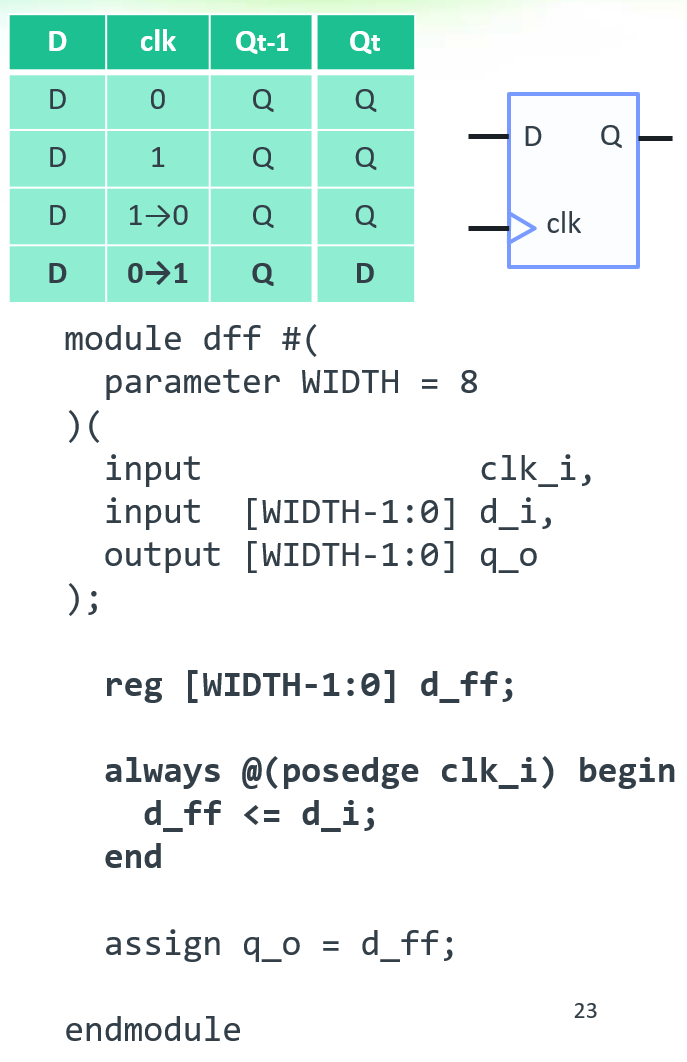
\includegraphics[width=\linewidth]{Learning/comb_logic.png}
        \caption{Картинка из презентации}
    \end{minipage}
\end{figure}

\begin{figure}[H]
    \centering
    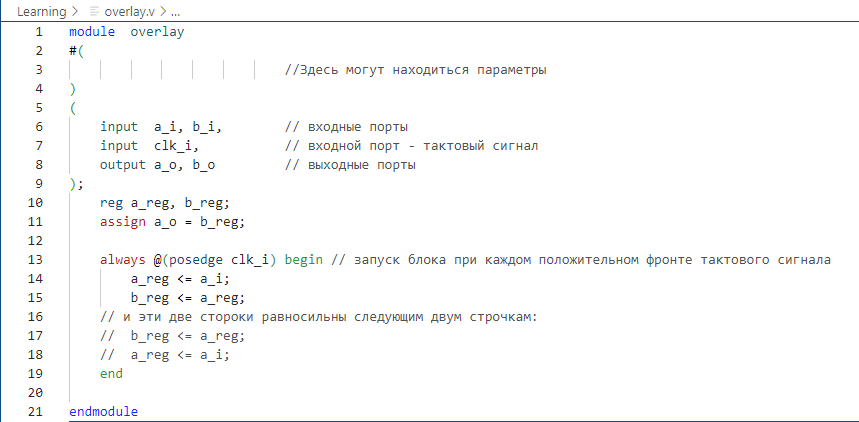
\includegraphics[width=1\linewidth]{Learning/overlay.png}
    \caption{\textbackslash Learning\textbackslash overlay.v}
\end{figure}

Здесь я хочу показать, что неблокирующие присваивания можно менять местами. Помимо простых рассуждений, хочу добавить результат обработки программы \textbf{Quartus Prime}. Это приложение от \textbf{Intel}, которое поддерживает ведение проектов на Verilog, поэтому считаю, что следующий аргумент будет достаточно весомым в области того, как нужно воспринимать код Verilog.

\begin{figure}[H]
    \centering
    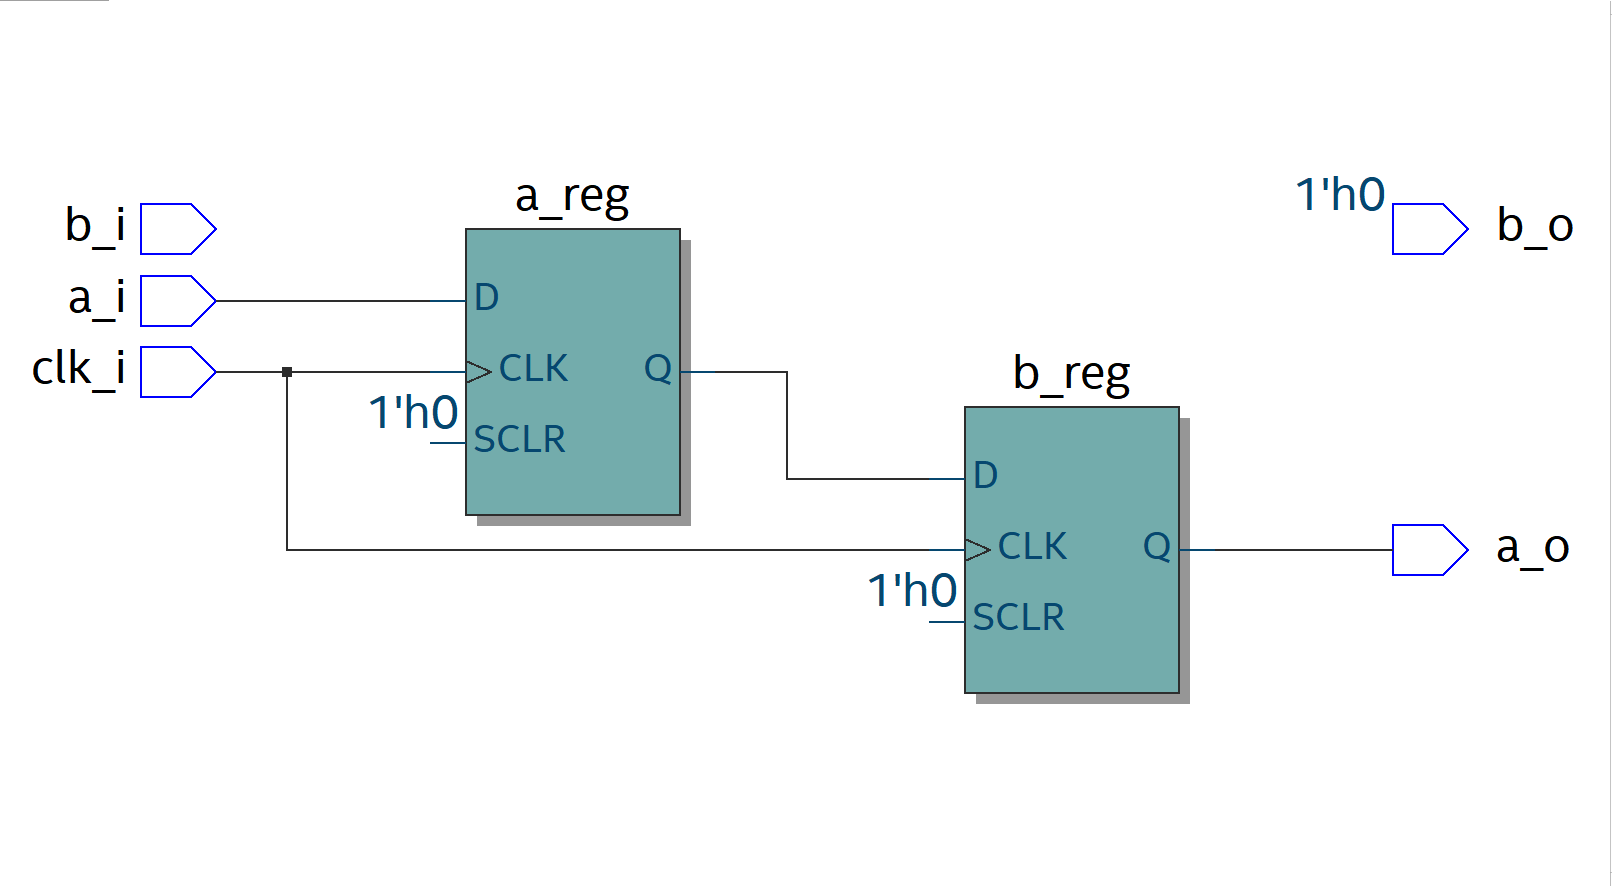
\includegraphics[width=1\linewidth]{Learning/RTL_overlay.png}
    \caption{Результат обработки файла \textbackslash Learning\textbackslash overlay.v}
\end{figure}

Действительно, как и было сказано ранее, неблокирующее присваивание ``<='' стоит рассматривать как DFF.

\begin{figure}[H]
    \centering
    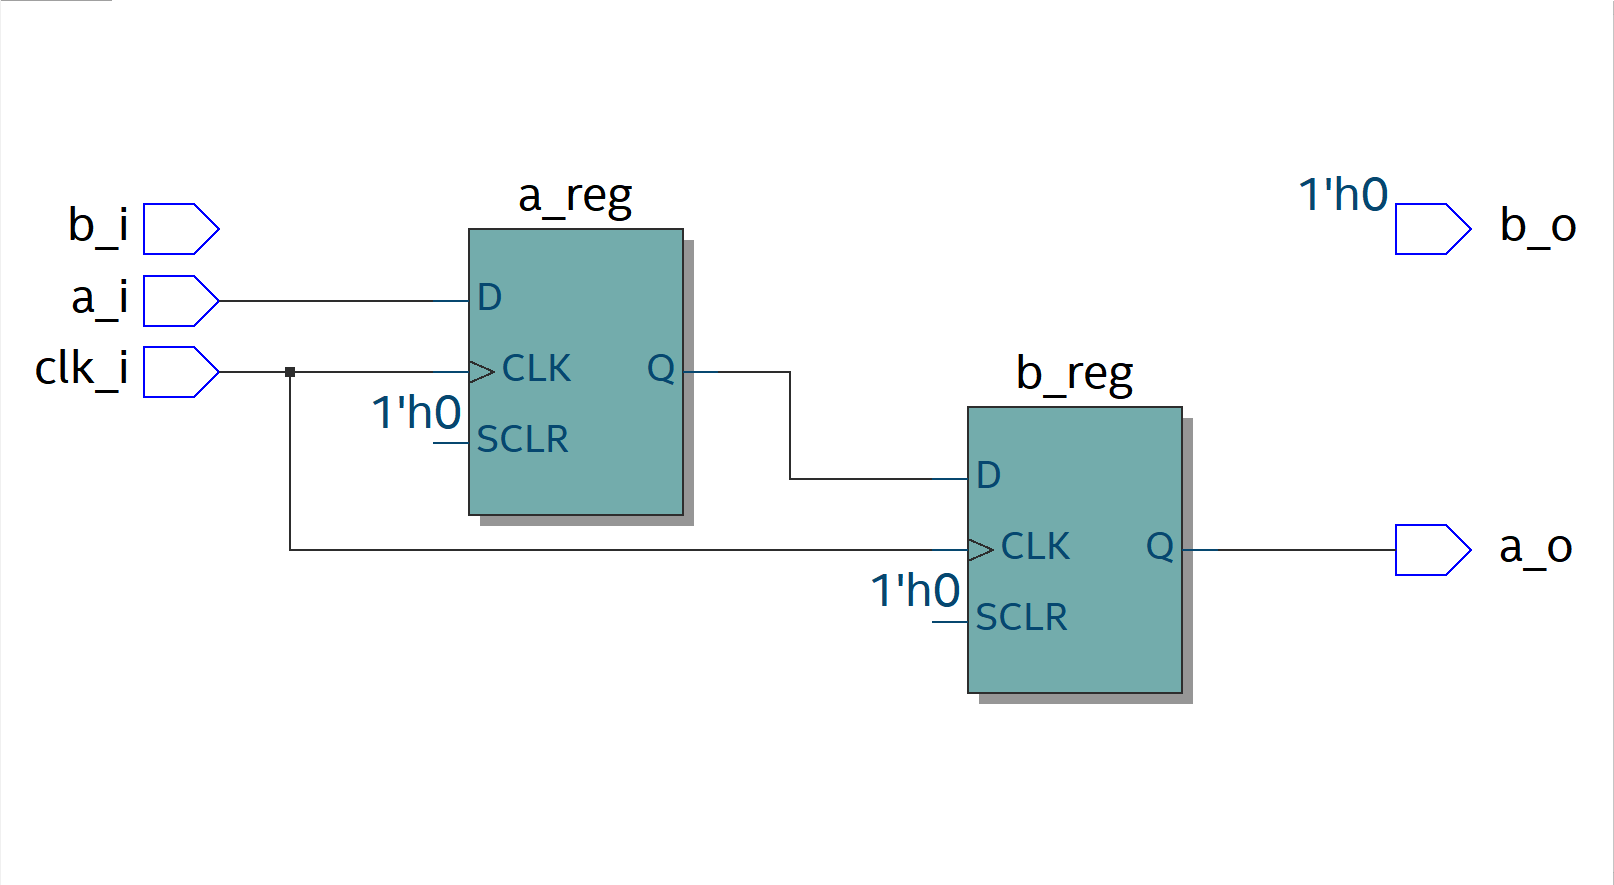
\includegraphics[width=1\linewidth]{Learning/RTL_overlay1.png}
    \caption{А это уже результат обработки того же файла, если поменять строки.}
\end{figure}

\begin{figure}[H]
    \begin{minipage}[t]{0.7\textwidth}
        \vspace{0pt} % Для точного выравнивания по верхнему краю
        Очень интересно. Несмотря на другой код, генерируется та же RTL схема. Хотя бы это уже говорит о том, что взаимное расположение строк не играет роли, но всё же, если генерируется некая схема, почему бы не разобраться в причине, почему же так выходит.
    \end{minipage}%
    \hfill
    \begin{minipage}[t]{0.25\textwidth}
        \vspace{0pt} % Для точного выравнивания по верхнему краю
        \centering
        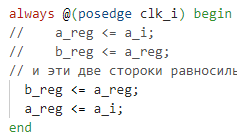
\includegraphics[width=\linewidth]{Learning/overlay_code.png}
    \end{minipage}
\end{figure}

\begin{figure}[H]
    \centering
    \begin{minipage}[t]{0.32\textwidth}
        \centering
        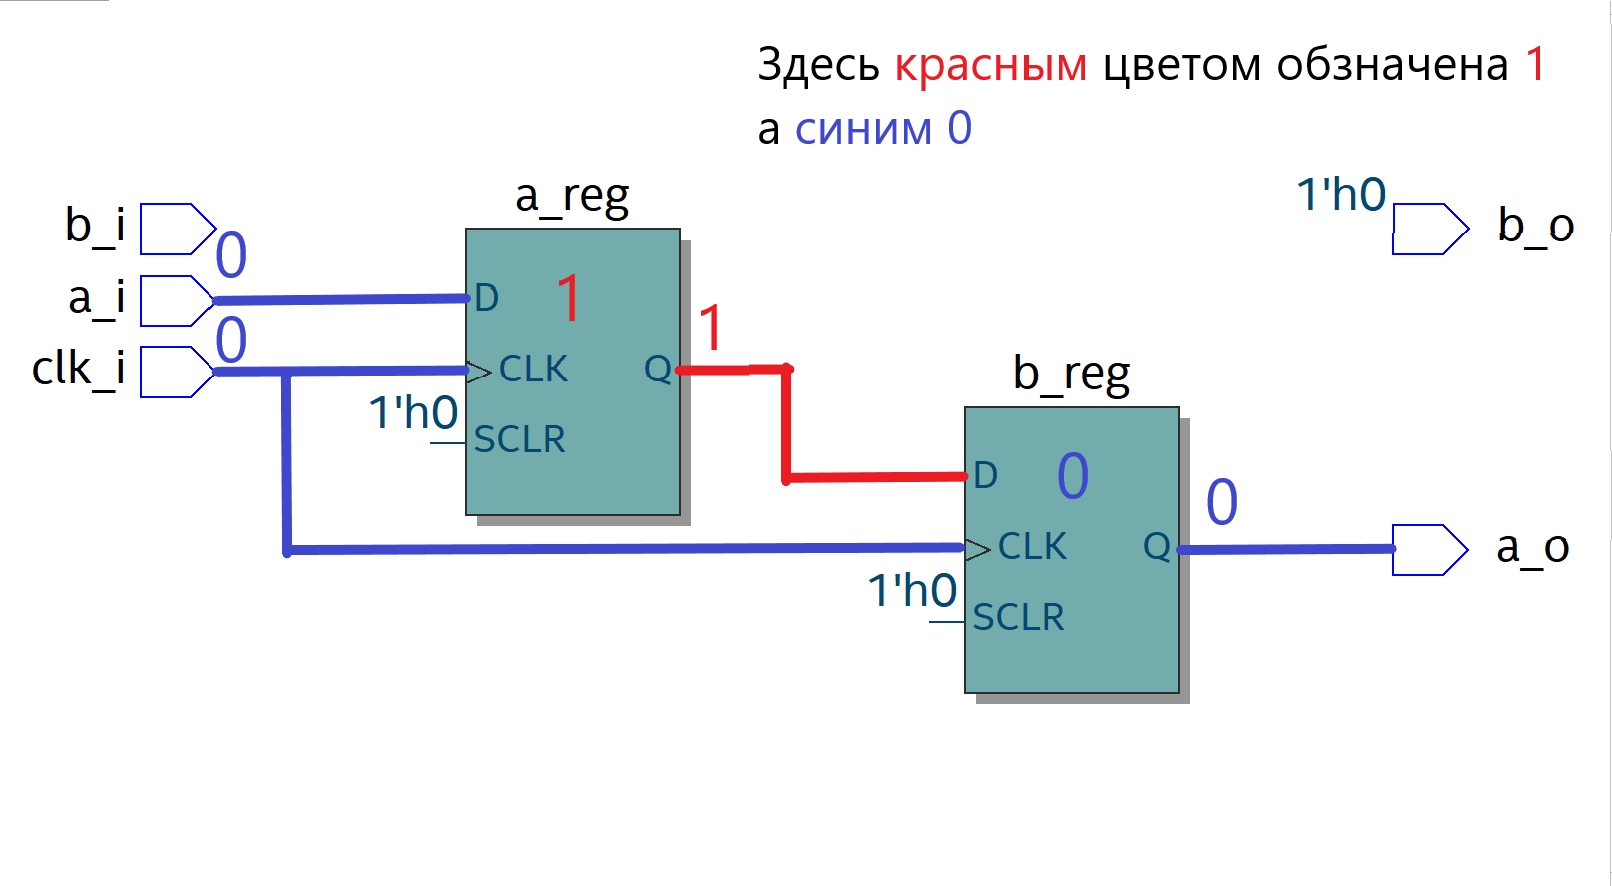
\includegraphics[width=\linewidth]{Learning/RTL1.png}
        \caption{Шаг 1}
        \label{fig:rtl1}
    \end{minipage}
    \hfill
    \begin{minipage}[t]{0.32\textwidth}
        \centering
        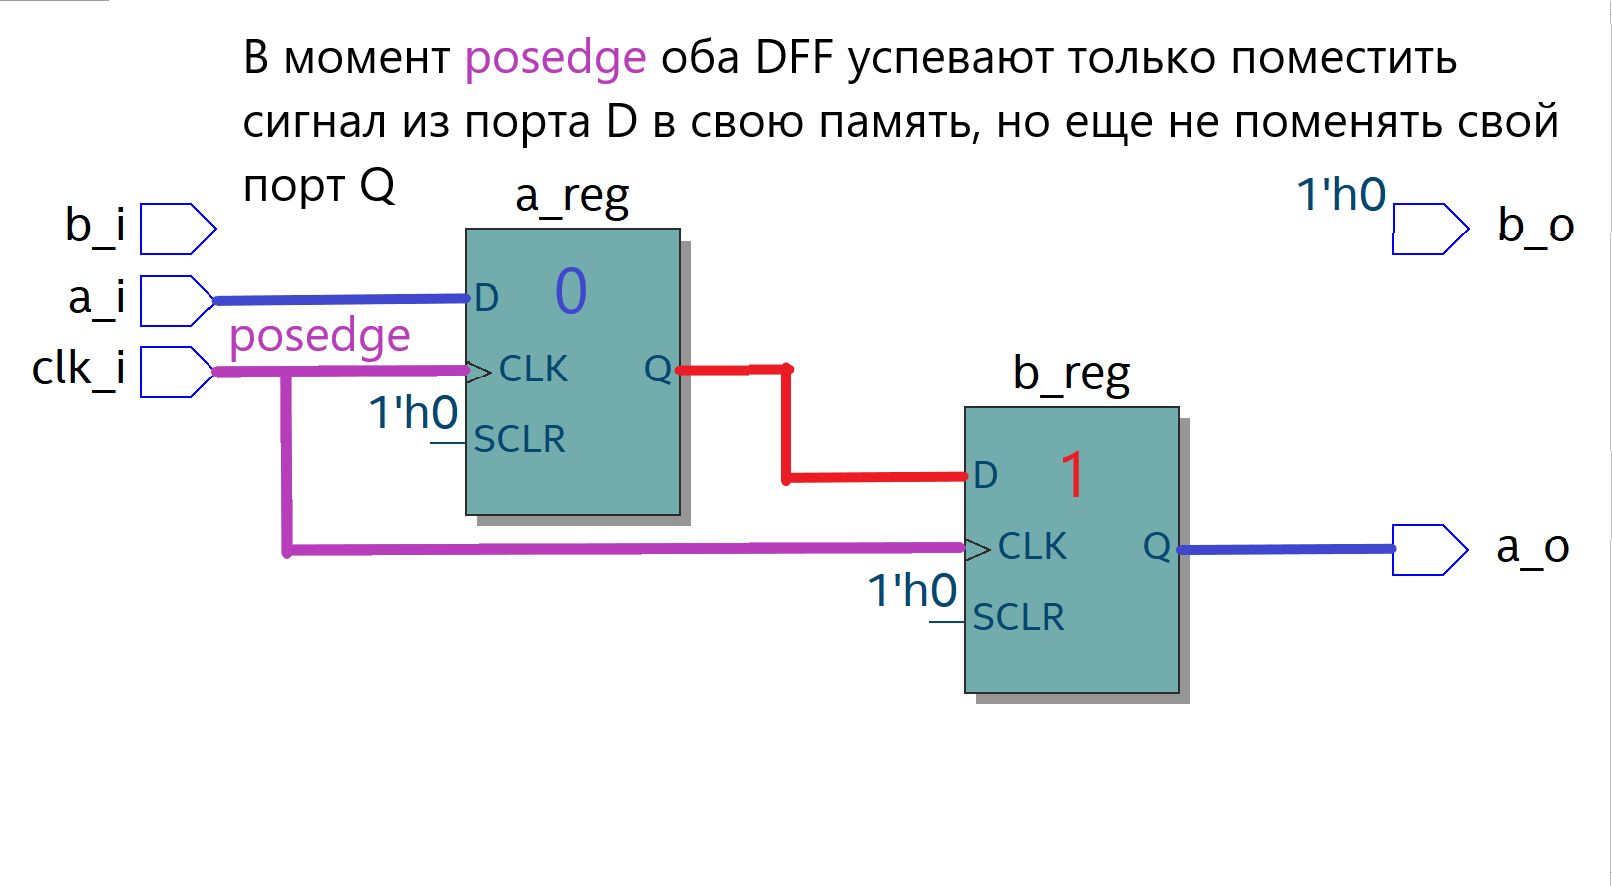
\includegraphics[width=\linewidth]{Learning/RTL2.png}
        \caption{Шаг 2}
        \label{fig:rtl2}
    \end{minipage}
    \hfill
    \begin{minipage}[t]{0.32\textwidth}
        \centering
        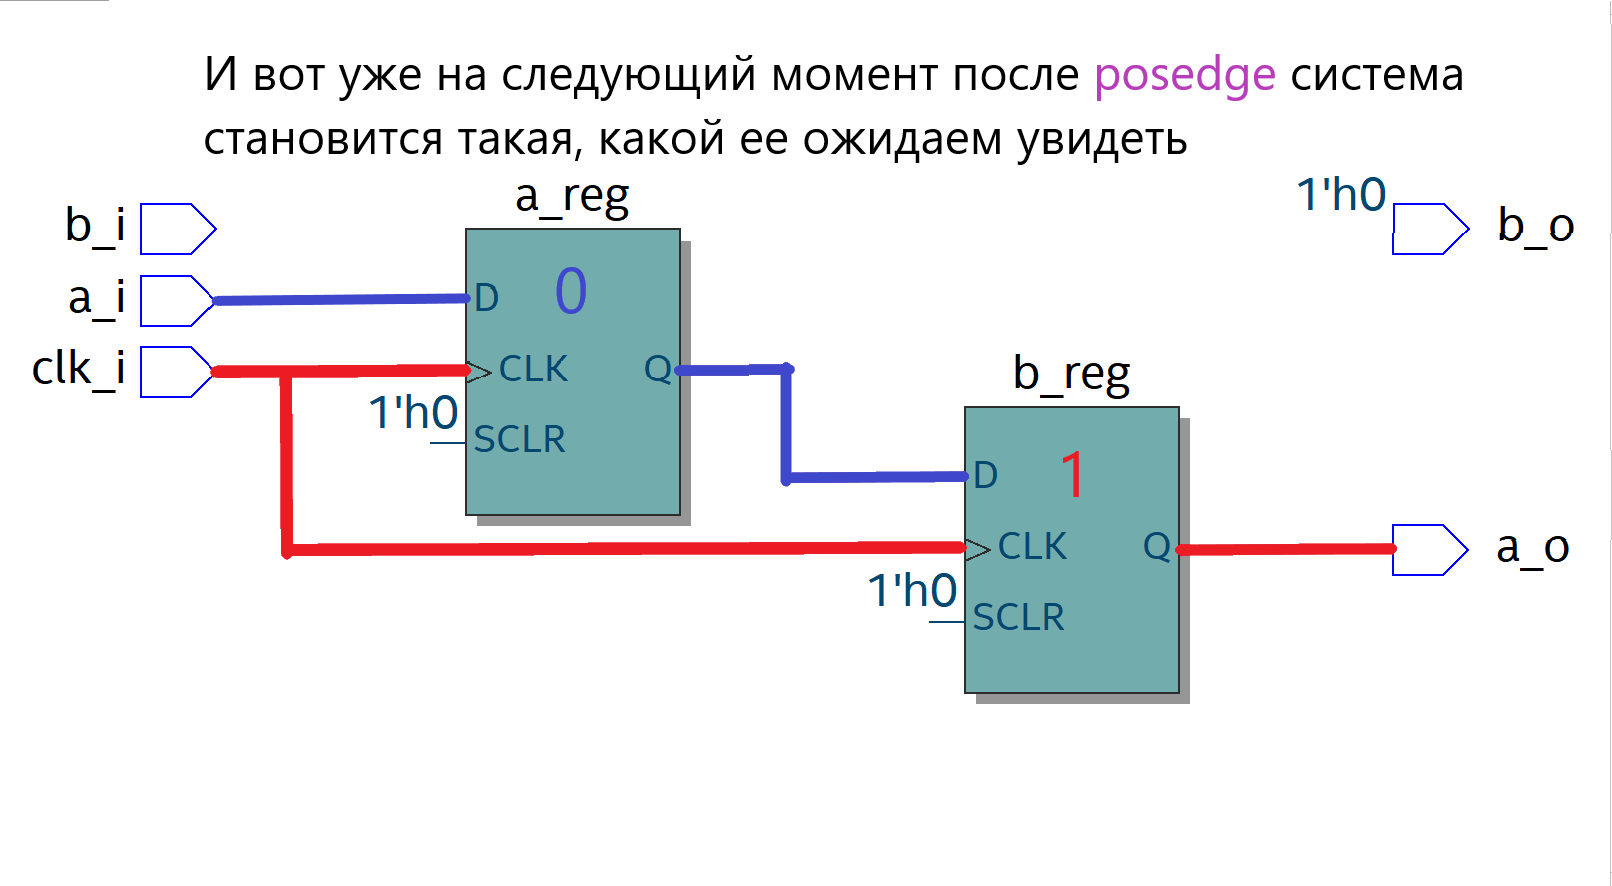
\includegraphics[width=\linewidth]{Learning/RTL3.png}
        \caption{Шаг 3}
        \label{fig:rtl3}
    \end{minipage}
\end{figure}

Считаю, на этом можно и остановиться в рассмотрении этих тем. 

\subsubsection{Testbench}

Чтобы удостовериться в работоспособности написанного кода, следует его проверить. С этим помогает так называемый \textbf{testbench}. 

Модули в Verilog можно сохранять, импортировать и использовать в других модулях. Таким образом, суть testbench заключается в том, чтобы проверяемый модуль полностью обернуть другим модулем, соединить соответствующие входные и выходные порты, и манипулируя временем и работой портов, проследить работу первого модуля. Оно же инстанцирование модуля.

Напишем тогда testbench для файла \textit{overlay.h}, чтобы рассмотреть его работу под новым углом.

\begin{figure}[H]
    \centering
    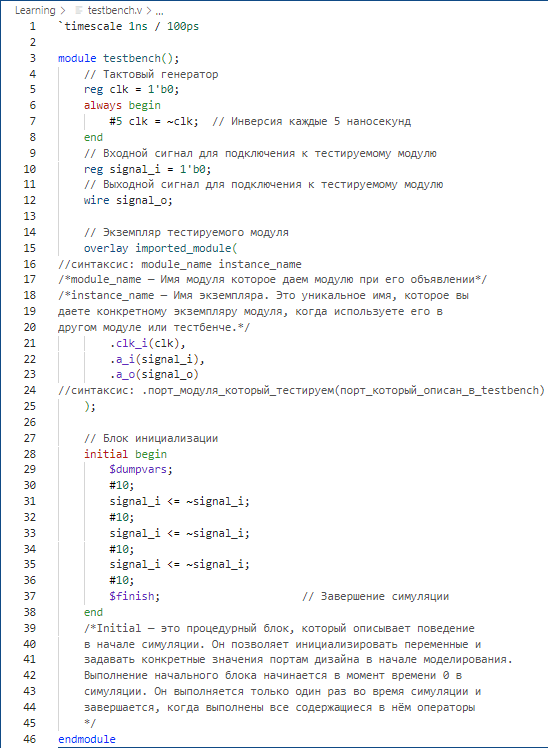
\includegraphics[width=1\linewidth]{Learning/TB_description.png}
    \caption{\textbackslash Learning\textbackslash testbench.v}
\end{figure}

Впрочем, в файле и на картинке описание достаточно подробное, в дополнительных описаниях нужды не вижу.

Можно запустить при помощи \textbf{Makefile} и проверить работу.
\begin{figure}[H]
    \centering
    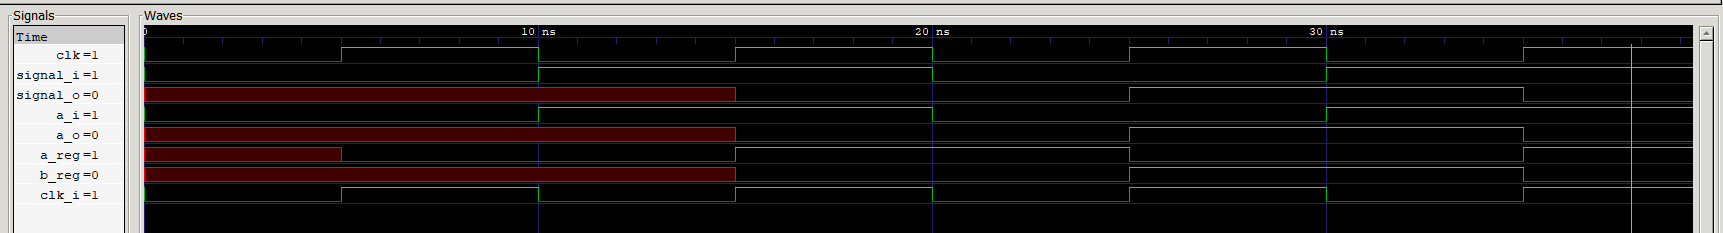
\includegraphics[width=1\linewidth]{Learning/TB.png}
\end{figure}
\textbf{Testbench} работает как и предполагалось. Супер!

\subsection{Сборка}

Знаний, описанных выше, достаточно для сбора АЛУ. Можно и приступать. 

Пошел генерал с внуком в цирк. До этого никогда в цирке не был. Там бегемот дрессированный по сцене бегает, клоуны валяются, поливаются из ведра, гимнасты на полотнах...
Генерал сидит красный весь, прям закипает, а потом как заорет командным голосом:

Для описания каждого из 8-ми операций не будем создавать отдельно 8 модулей, так как эти операции уже описаны в стандартной библиотеке, да и код не охота раздувать.

\begin{figure}[H]
    \centering
    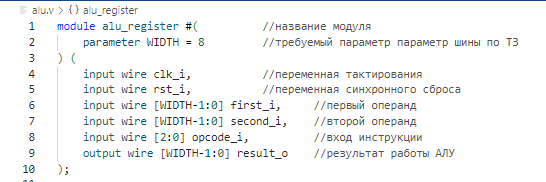
\includegraphics[width=1\linewidth]{Final/variables.png}
\end{figure}

Здесь описали входные и выходные порты, которые были описаны.

\begin{figure}[H]
    \centering
    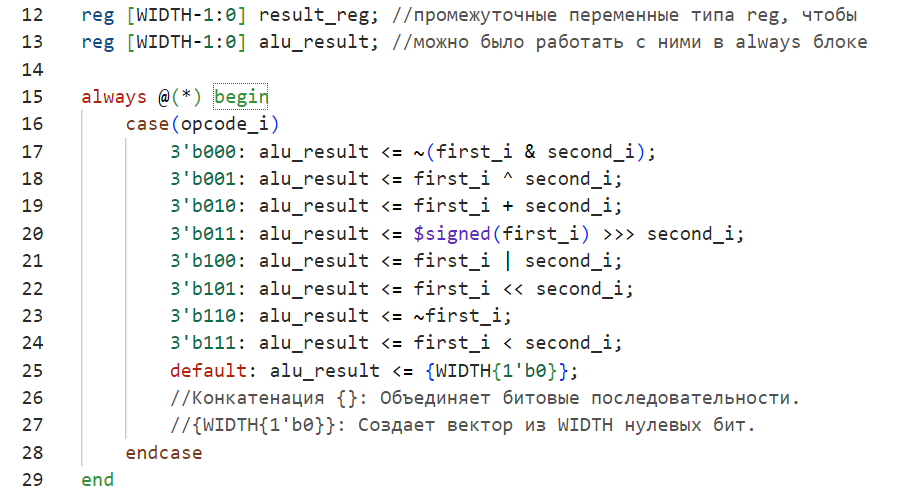
\includegraphics[width=1\linewidth]{Final/opers.png}
\end{figure}

Структура \textbf{case} подобна структурам \textbf{switch} в других языках программирования, считаю что понимание этого абзаца интуитивно.

Стандартом языка предусмотрены специальные системные функции $\$$ signed() и $\$$ unsigned(). Эти функции по своей сути являются директивами компилятору, они говорят ему, как он должен интерпретировать выражение. При этом разрядность входного выражения не меняется.

$\$$signed – возвращаемое значение знаковое, $\$$unsigned – возвращаемое значение беззнаковое.

\begin{figure}[H]
    \centering
    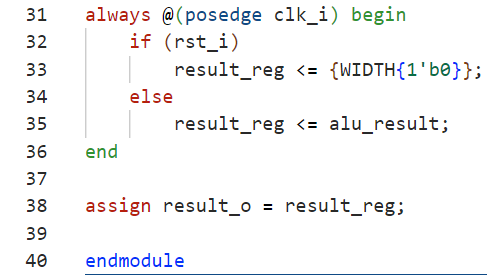
\includegraphics[width=0.5\linewidth]{Final/end.png}
\end{figure}

Здесь прописываем работу тактового сигнала и сигнала сброса. По ТЗ сказано реализовать синхронный сброс, а значит, приоритет проверки сигнала тактирования выше, и только внутри этого цикла  можно установить ветвление. И в конце концов выдаем сигнал регистра на выход АЛУ.

Замечательно. Посмотрим, как его нарисует Quartus.

\begin{figure}[H]
    \centering
    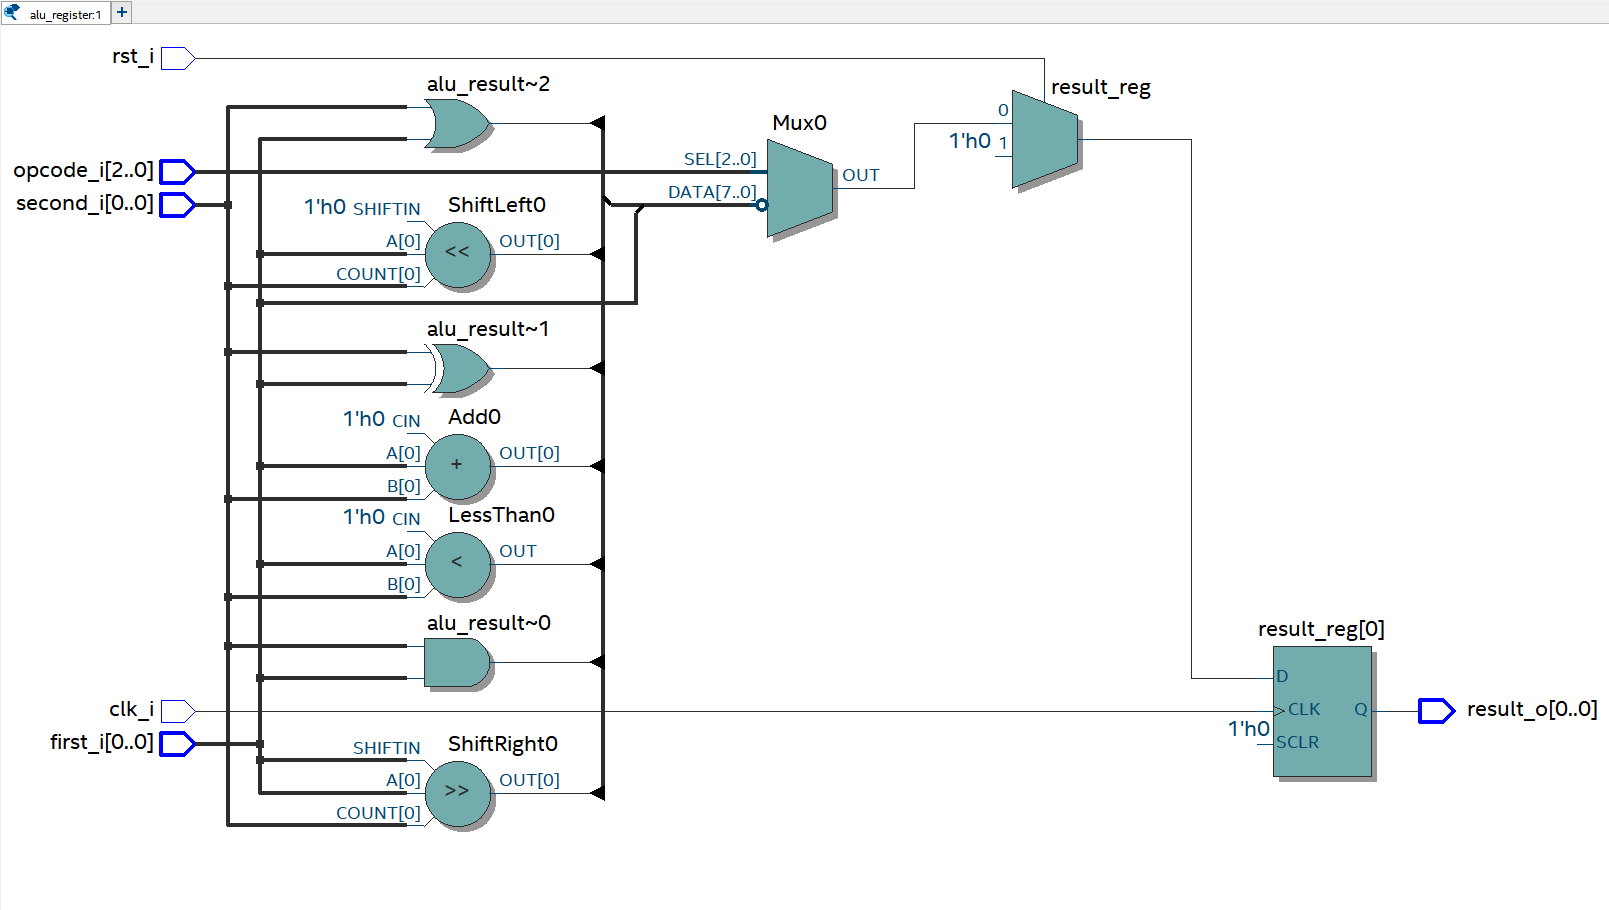
\includegraphics[width=1\linewidth]{Final/Quartus_alu.png}
    \caption{Схема при WIDTH = 1}
\end{figure}

Фантастика. Схема соответствует ожиданиям и схожа с принципиальной схемой на стр.2.

Теперь можно написать testbench для проверки модуля, как того требует ТЗ. Ничего интересного в этом коде нет, просто поочередно проверяем функциональность каждого элемента.

\begin{figure}[H]
    \centering
    \includegraphics[width=1\linewidth]{Final/tb.png}
\end{figure}

Все системы работают корректно. Результат появляется только по положительному фронту тактирующего сигнала, как и требуется в ТЗ. Сигнал сброса обнуляет выходную шину, но только по фронту тактирующего сигнала, как и требуется в ТЗ. Каждая логическая и арифметическая операция соответствует своему коду и выполняет свои функции, как и требуется в ТЗ. 

Когда все аспекты рассмотрены, можно начать написание "формального отчета".

\section{Формальный отчет}
\begin{enumerate}
    \item Выполнил: Комиссаров Данил Андреевич.
    \item Студент группы Б01-304.
    \item Первый вариант задания. Арифметико-логическое устройство (ALU).
    \item Контакты: komissarov.da@phystech.edu
    \item Модуль alu\_register выполняет арифметические и логические операции над двумя входными операндами (first\_i, second\_i) в соответствии с кодом операции (opcode\_i). Результат операции сохраняется в регистр и выводится на порт result\_o на следующий такт. Модуль поддерживает синхронный сброс, обнуляющий регистр при активации сигнала rst\_i.
    \item
\begin{figure}[H]
    \centering
    \includegraphics[width=1\linewidth]{Formal/АЛУ1.png}
\end{figure}
    \item
Параметр	WIDTH		\\
Описание	Разрядность операндов\\
Допустимые значения Целое число больше или равно 1\\
    \item
    \begin{table}[H]
\centering
\label{tab:ports}
\begin{tabular}{|l|c|l|p{6cm}|}
\hline
\textbf{Название} & \textbf{Ширина} & \textbf{Направление} & \textbf{Описание} \\ \hline
clk\_i    & 1      & Вход    & Тактовый сигнал \\ \hline
rst\_i    & 1      & Вход    & Синхронный сброс (активный уровень — 1) \\ \hline
first\_i  & WIDTH  & Вход    & Первый операнд \\ \hline
second\_i & WIDTH  & Вход    & Второй операнд \\ \hline
opcode\_i & 3      & Вход    & Код операции \\ \hline
result\_o & WIDTH  & Выход   & Результат операции \\ \hline
\end{tabular}
\end{table}
\item
Тактирование и сброс\\
Тактирование: По положительному фронту сигнала clk\_i.\\
Сброс: Синхронный (активный уровень — 1).\\
При активации rst\_i регистр обнуляется на следующем такте.
\item 
Тестирование
Сценарий тестирования:
\begin{enumerate}
\item Сброс: Проверка обнуления регистра при активации rst\_i.\\
\textbf{Проверка операций:}
\item Побитовое НЕ-И (opcode\_i = 000).
\item Исключающее ИЛИ (001).
\item Сложение (010).
\item Арифметический сдвиг вправо (011).
\item Побитовое ИЛИ (100).
\item Логический сдвиг влево (101).
\item Побитовое НЕ (110).
\item Сравнение (111).
\item Граничные случаи:
\item Переполнение при сложении.
\item Сдвиг на значение, превышающее разрядность.
\item Задержка вывода: Убедиться, что результат появляется через такт.
\item Сброс: Снова обнуление регистра.
\end{enumerate}
\item В папке будет находиться Makefile, чтобы запустить все файлы в папке, введите в консоль \textit{make run}, чтобы отчистить папку от результатов компиляции, введите \textit{make clean}.
\item
\begin{figure}[H]
    \centering
    \includegraphics[width=1\linewidth]{Formal/tb.png}
\end{figure}
\end{enumerate}

На этом пожалуй можно и закончить. Наверное я уделил слишком много внимания несущественным аспектам, в то время, когда некоторые фундаментальные принципы были упущены, но это было интересно. 

\end{document}
